% LaTeX source for "OpenStack Beginner's Guide"
% Copyright (c)  2014.

% Permission is granted to copy and redistribute the material in any medium or format remix, transform, and build upon the material
% for any purpose, even commercially under the Creative Commons - Attribution-Sharealike International
% License,Version 4.0. A copy of the license can be found at creativecommons.org

%
\documentclass[10pt]{book}
\usepackage[a4paper, hmarginratio=3:2,vmarginratio=3:2]{geometry}
%\usepackage[paperwidth=6in, paperheight=9in, width=4.5in, height=7.5in,
%  hmarginratio=3:2,vmarginratio=3:2]{geometry}
% \usepackage[paperwidth=8.27in,paperheight=11.69in,
%  width=5.9in,height=9.64in,
%  hmarginratio=3:2,vmarginratio=3:2]{geometry}
\usepackage{fancyhdr}
\usepackage{graphicx}
\usepackage{epsfig}
\usepackage{makeidx}
\usepackage{hyperref}
\usepackage{listings}
\usepackage{color}
\usepackage{textcomp}
\usepackage[ final ]{pdfpages}
\usepackage[cc]{titlepic}
\usepackage{multirow} % table multirow multicolumn etc..
\usepackage{rotating} % table rotation
\usepackage[dvipsnames,table]{xcolor} % table colors ;-)
%\usepackage[usenames,dvipsnames]{color} % table color duh.. x-(
\usepackage{booktabs} % Professional Tables



\pssilent

\sloppy

% margins for A4, mirroring
% \setlength{\oddsidemargin}{1.0in}
% \setlength{\evensidemargin}{0.5in}

% dimensions for b5paper
%\setlength{\topmargin}{-0.375in}
%\setlength{\oddsidemargin}{0.0in}
%\setlength{\evensidemargin}{0.0in}

% dimensions for 8.5 x 11
%\setlength{\topmargin}{0.625in}
%\setlength{\oddsidemargin}{0.875in}
%\setlength{\evensidemargin}{0.875in}

\setlength{\headsep}{3ex}
%\setlength{\textheight}{9.64in}

\setlength{\parindent}{0.0in}
\setlength{\parskip}{1.7ex plus 0.5ex minus 0.5ex}
\renewcommand{\baselinestretch}{1.02}

% see LaTeX Companion page 62
\setlength{\topsep}{-0.0\parskip}
\setlength{\partopsep}{-0.5\parskip}
\setlength{\itemindent}{0.0in}
\setlength{\listparindent}{0.0in}

% see LaTeX Companion page 26
% these are copied from /usr/local/teTeX/share/texmf/tex/latex/base/book.cls
% all I changed is afterskip

\makeatletter
\renewcommand{\section}{\@startsection 
    {section} {1} {0mm}%
    {-3.5ex \@plus -1ex \@minus -.2ex}%
    {0.7ex \@plus.2ex}%
    {\normalfont\Large\bfseries}}
\renewcommand\subsection{\@startsection {subsection}{2}{0mm}%
    {-3.25ex\@plus -1ex \@minus -.2ex}%
    {0.3ex \@plus .2ex}%
    {\normalfont\large\bfseries}}
\renewcommand\subsubsection{\@startsection {subsubsection}{3}{0mm}%
    {-3.25ex\@plus -1ex \@minus -.2ex}%
    {0.3ex \@plus .2ex}%
    {\normalfont\normalsize\bfseries}}
\makeatother

\newcommand{\beforefig}{\vspace{1.3\parskip}}
\newcommand{\afterfig}{\vspace{-0.2\parskip}}

\newcommand{\beforeverb}{\vspace{0.6\parskip}}
\newcommand{\afterverb}{\vspace{0.6\parskip}}

\newcommand{\adjustpage}[1]{\enlargethispage{#1\baselineskip}}

% all hyperlinks to appear in blue text and remove boxes for hyperlinks
\hypersetup{%
    pdfborder = {0 0 0},
    colorlinks = true,
    linkcolor = blue,
    urlcolor = blue
}

% code and command highlighting
\definecolor{listinggray}{gray}{0.9}
\definecolor{lbcolor}{rgb}{0.9,0.9,0.9}
\lstset{
	backgroundcolor=\color{lbcolor},
	tabsize=4,
	rulecolor=,
        basicstyle=\scriptsize,
        upquote=true,
        aboveskip={1.5\baselineskip},
	columns=fullflexible,         
	%columns=fixed,
        showstringspaces=false,
        extendedchars=true,
        breaklines=true,
        prebreak = \raisebox{0ex}[0ex][0ex]{\ensuremath{\hookleftarrow}},
        frame=single,
        showtabs=false,
        showspaces=false,
        showstringspaces=false,
        identifierstyle=\ttfamily,
        keywordstyle=\color[rgb]{0,0,1},
        commentstyle=\color[rgb]{0.133,0.545,0.133},
        stringstyle=\color[rgb]{0.627,0.126,0.941},
}

% Note: the following command seems to cause problems for Acroreader
% on Windows, so for now I am overriding it.

\let\origdoublepage\cleardoublepage
\newcommand{\clearemptydoublepage}{%
  \clearpage
  {\pagestyle{empty}\origdoublepage}%
}


%\newcommand{\clearemptydoublepage}{\newpage{\pagestyle{empty}\cleardoublepage}}

%\renewcommand{\clearemptydoublepage}{\cleardoublepage}

\newcommand{\blankpage}{\pagestyle{empty}\vspace*{1in}\newpage}
\renewcommand{\blankpage}{\vspace*{1in}\newpage}

\pagestyle{fancyplain}

\renewcommand{\chaptermark}[1]{\markboth{#1}{}}
\renewcommand{\sectionmark}[1]{\markright{\thesection\ #1}{}}

\lhead[\fancyplain{}{\bfseries\thepage}]%
      {\fancyplain{}{\bfseries\leftmark}}
\rhead[\fancyplain{}{\bfseries\leftmark}]%
      {\fancyplain{}{\bfseries\thepage}}

%\cfoot{OpenStack Beginner's Guide: Ubuntu Trusty Edition}

\cfoot{\fancyplain{}{OpenStack Beginner's Guide: Ubuntu Trusty Edition}}



\renewcommand{\footrulewidth}{\headrulewidth}


% turn off the rule under the header
%\setlength{\headrulewidth}{0pt}

% the following is a brute-force way to prevent the headers
% from getting transformed into all-caps
\renewcommand\MakeUppercase{}

\makeindex




\begin{document}

\frontmatter

\thispagestyle{empty}
%-top cover--------------------------------------------------
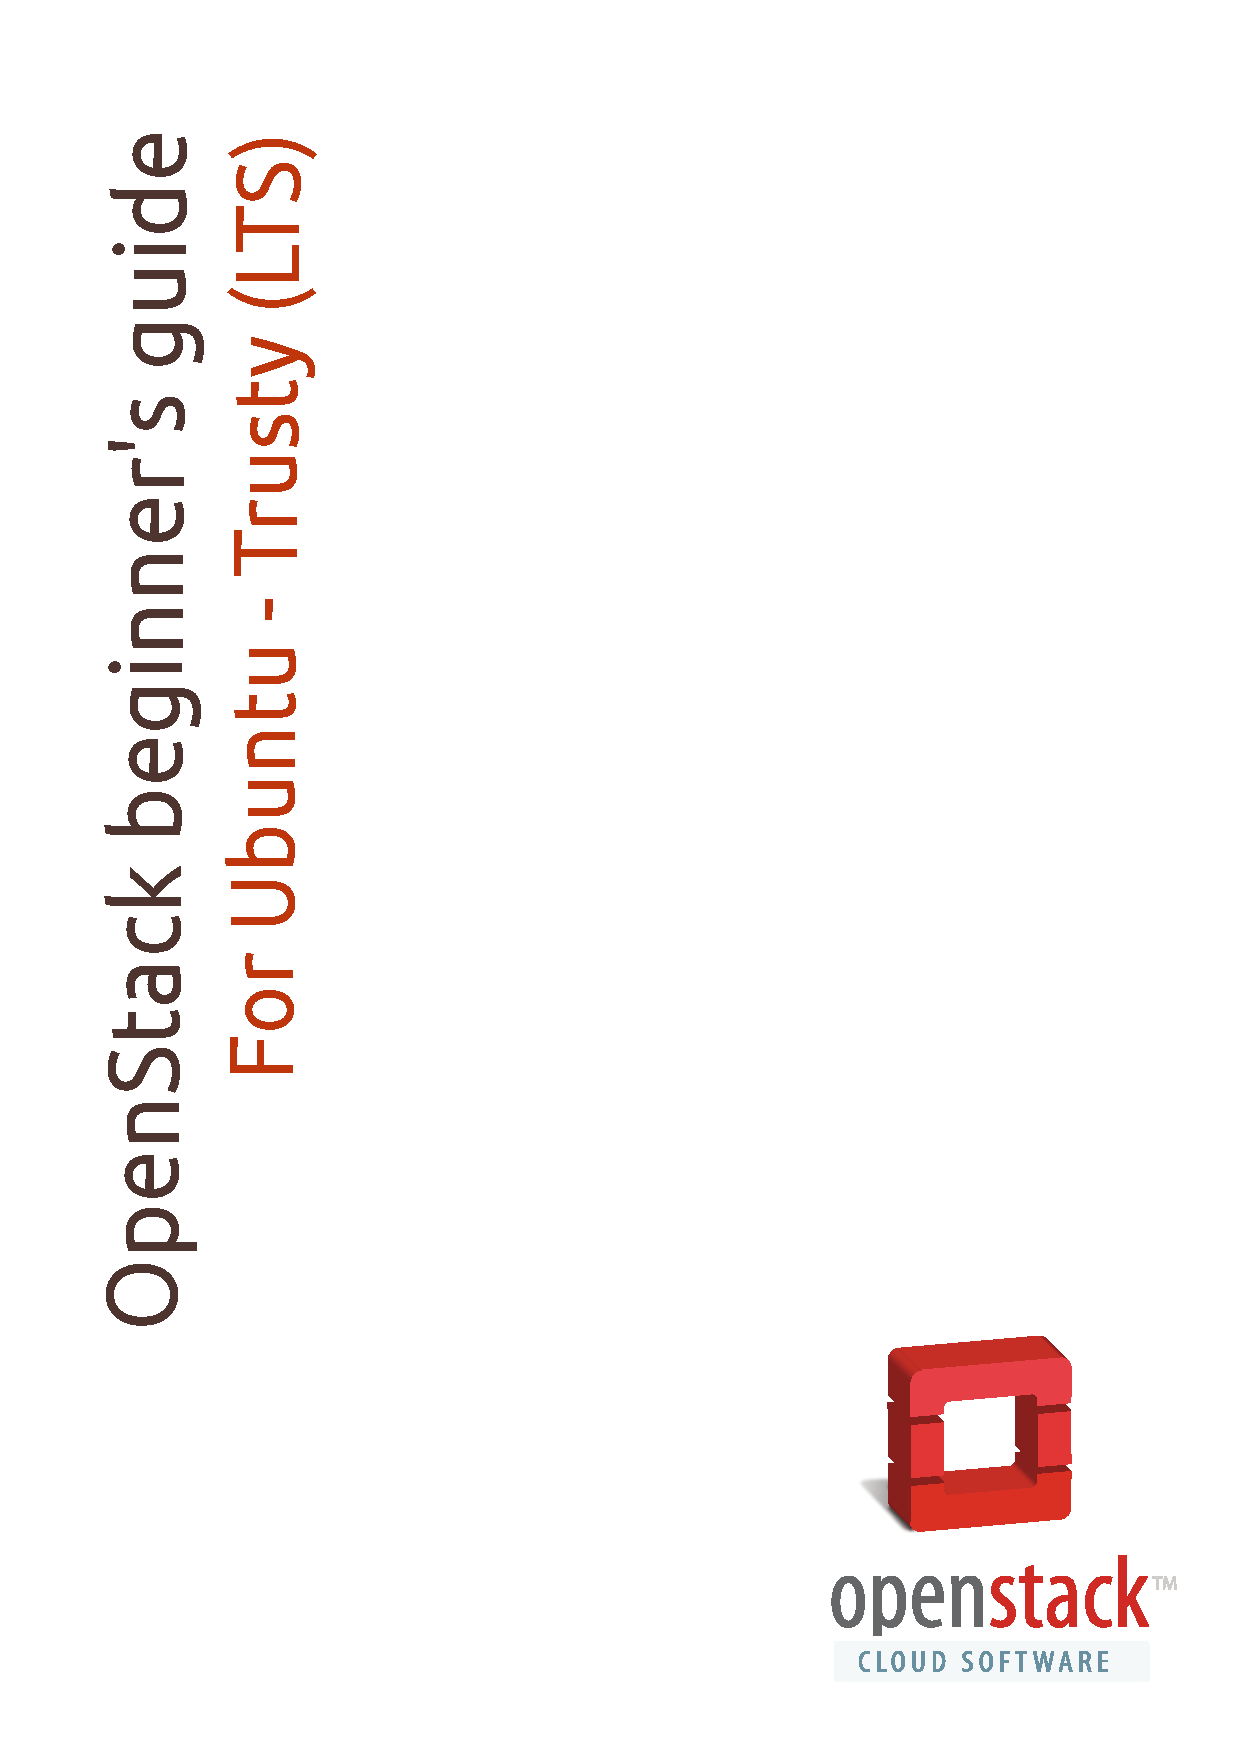
\includepdf[]{../images/cover.pdf}

%\hspace*{-1in}
%\vspace*{-2in}
%\begin{figure}
%	\begin{center}
%		\includegraphics[width=\paperwidth, height=\paperheight]{../images/bookcover}
%	\end{center}
%\end{figure]
%--title page--------------------------------------------------

\clearemptydoublepage


\pagebreak
\thispagestyle{empty}
\begin{center}
{\huge OpenStack Beginner's Guide }
\vspace{0.2cm}
{\Large \\(for Ubuntu - Trusty)}
\vspace{0.2cm}
{\large \\v4.2, 10 Nov 2014}
%\begin{flushright}
\vspace{2in}
{\large
\\
Akilesh K\\
Johnson D\\
Yogesh G\\
}
%\end{flushright}
\end{center}
\vspace{0.1in}
\begin{figure}[h!]
	\begin{center}
		\href{http://www.openstack.org/}{
\includegraphics[width=0.3\textwidth]{../images/openstacklogo}}
		\label{openstack logo}
	\end{center}
\end{figure}
%--copyright--------------------------------------------------

\pagebreak
\thispagestyle{empty}
\begin{flushleft}
\vspace{1in}
% \centering
\begin{center}
{\huge OpenStack Beginner's Guide } 
\vspace{0.2cm}
{\Large \\(for Ubuntu - Trusty)}
\vspace{0.2cm}
{\large \\v4.2, 10 Nov 2014}

\vspace{0.05in}
\end{center}

\vspace{0.05in}
% \centering

\vspace{1in}
'Ubuntu', the Ubuntu Logo and 'Canonical' are registered trademarks of  
\href{http://www.canonical.com/}{Canonical}. Read Canonical's trademark policy
\href{http://www.ubuntu.com/aboutus/trademarkpolicy}{here}.

\vspace{0.1in}
'OpenStack' and the OpenStack Logo are registered trademarks of  
\href{http://www.openstack.org/}{OpenStack}. Read OpenStack's trademark policy
\href{http://www.openstack.org/brand/openstack-trademark-policy/}{here}.

\vspace{0.1in}
All other trademarks mentioned in the book belong to their respective owners.


\vspace{0.1in}
This book is aimed at making it easy/simple for a beginner to build and maintain a private cloud using OpenStack. This book will be updated periodically based on the suggestions, ideas, corrections, etc., from readers. 

% \centering
\vspace{0.1in}
\textbf{Mail Feedback to}: \href{mailto:books@pinlabs.in}{books@pinlabs.in} \\

\vspace{0.1in}
\textbf{Please report bugs in the content of this book at }: \href{https://github.com/eternaltyro/openstack-beginners-guide}{https://github.com/eternaltyro/openstack-beginners-guide} and we will try to fix them as early as possible and incorporate them in to the next version of the book.\\


\vspace{0.1in}
Released under Creative Commons - Attribution-ShareAlike 4.0 International license.\\
\vspace{0.1in}
\href{http://creativecommons.org/licenses/by-sa/4.0/}{A brief description of the license}\\
\vspace{0.1in}
\href{http://creativecommons.org/licenses/by-sa/4.0/legalcode}{A more detailed license text}

\end{flushleft} 
\vspace{0.5in}

\begin{figure}[h!]
	\begin{center}
\href{http://creativecommons.org/licenses/by-sa/4.0/}{
\includegraphics[scale=0.50]{../images/license}}
%		
\includegraphics[width=155pt,height=43pt]{../images/license}
		\label{License}
	\end{center}
\end{figure}

%-----------------------------------------------------------------

% LaTeX source for "OpenStack Beginner's Guide"
% Copyright (c)  2014  pinlabs.in.

% Permission is granted to copy, distribute and/or modify this document under
% the terms of the GNU Free Documentation License, Version 1.1  or any later
% version published by the Free Software Foundation; with the Invariant
% Sections being "Contributor List", "Forward", and "Preface", with no
% Front-Cover Texts, and with no Back-Cover Texts. A copy of the license is
% included in the section entitled "GNU Free Documentation License".

% This distribution includes a file named fdl.tex that contains the text of the
% GNU Free Documentation License.  If it is missing, you can obtain it from
% www.gnu.org or by writing to the Free Software Foundation, Inc.,
% 59 Temple Place - Suite 330, Boston, MA 02111-1307, USA.
%
\chapter{Preface} 

\section*{About this guide}
The idea of OpenStack Beginner's Guide came from OpenStack cactus release, during that time we had limited documentation available. Our initial contributors were Murthyraju Manthena, Kiran Murari, Suseendran RB, Yogesh G, Atul Jha and Johnson D. We released this book updating every version and adding newer components. Later on this book got merged with official OpenStack documentaion. We thought we still need to maintain this book for our reference and hence we are releasing the book for Icehouse version on Ubuntu 14.04 LTS.

\section*{Target Audience}
Our aim has been to provide a guide for a beginners who are new to OpenStack. Good familiarity with virtualization is assumed, as troubleshooting OpenStack related problems requires a good knowledge of virtualization. Similarly, familiarity with Cloud Computing concepts and terminology will be of help. Prior exposure to AWS API and/or tools is not mandatory, though such exposure will accelerate the learning process greatly.

\section*{Acknowledgement}
Most of the content has been borrowed from web resources like manuals, documentation, white papers etc. from OpenStack and Canonical; numerous posts on forums and discussions on OpenStack IRC Channel. We would like to thank all the authors of these resources.

\section*{License}
Attribution-ShareAlike 4.0 International. For the full version of the license text, please refer to
\url{http://creativecommons.org/licenses/by-sa/4.0/legalcode} and
\url{http://creativecommons.org/licenses/by-sa/4.0/} for a shorter description.

\section*{Feedback}
We would really appreciate your feedback. We will enhance the book on an ongoing basis based on your feedback. Please mail your feedback to 
\href{mailto:books@pinlabs.in}{books@pinlabs.in}.

\vspace{0.25in}
%\begin{flushright}
%Pinlabs.in Team\\
%pinlabs.in\\
%\end{flushright}


\clearemptydoublepage

% The following lines add a little extra space to the column
% in which the Section numbers appear in the table of contents




\end{document}
